\section{Conclusions}
	\begin{frame}{Author's Conclusions}
		\begin{itemize}
			\item[$\bullet$] Enhancements provided by adiabatic computers for solving \textbf{NP}-Hard or \textbf{NP}-Complete problems
			\item[$\bullet$] Promising result for Quantum Machine Learning
			\item[$\bullet$] The approach targets the global solution of the training problem \textbf{better} than the classic alternatives
			\item[$\bullet$] The \textbf{D-Wave 2000Q} machine
			\item[$\bullet$] Quantum approach partitions data with similar accuracy to the classical approaches
			\item[$\bullet$] The approach assumes viability as the quantum hardware improves
		\end{itemize}
	\end{frame}

	\begin{frame}{Future Works}
		\begin{itemize}
			\item[$\bullet$] Bring the QUBO formulation to the generic k-means training problem
			\item[$\bullet$] Use elements of the approach to formulate quantum algorithms for similar clustering models
			\begin{itemize}
				\item[$\circ$] k-medoids clustering
				\item[$\circ$] fuzzy C-means clustering
			\end{itemize}
			\item[$\bullet$] Cluster larger datasets 
		\end{itemize}
	\end{frame}

\section{Critical View}
	\begin{frame}[allowframebreaks]{Our Conclusions}
		\textbf{Can we cluster larger datasets on Advantage?}
		\begin{center}
			\begin{minipage}{0.5\textwidth}
				D-Wave 2000Q
				\begin{itemize}
					\item[$\bullet$] 2048 qubits
					\item[$\bullet$] 6,016 couplers
					\item[$\bullet$] 128,472 JJs
				\end{itemize}
				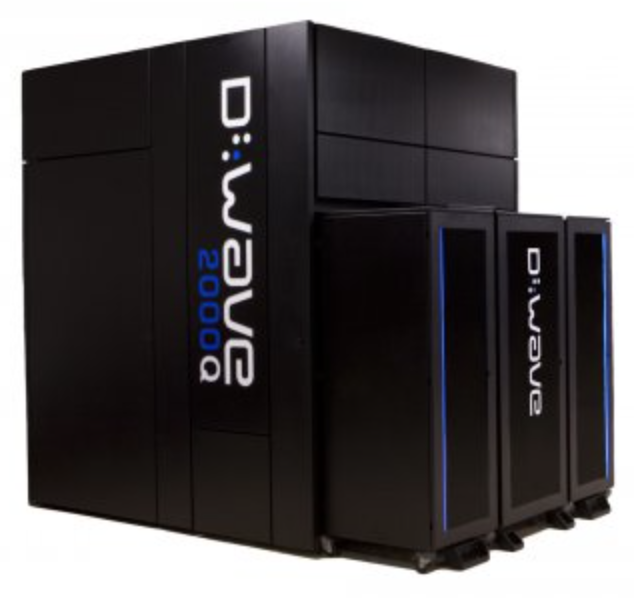
\includegraphics[scale=0.3]{2000Q.png}
			\end{minipage}~
			\begin{minipage}{0.5\textwidth}
				Advantage
				\begin{itemize}
					\item[$\bullet$] 5640 qubits
					\item[$\bullet$] 40,484 couplers
					\item[$\bullet$] 1,030,000 JJs
				\end{itemize}
				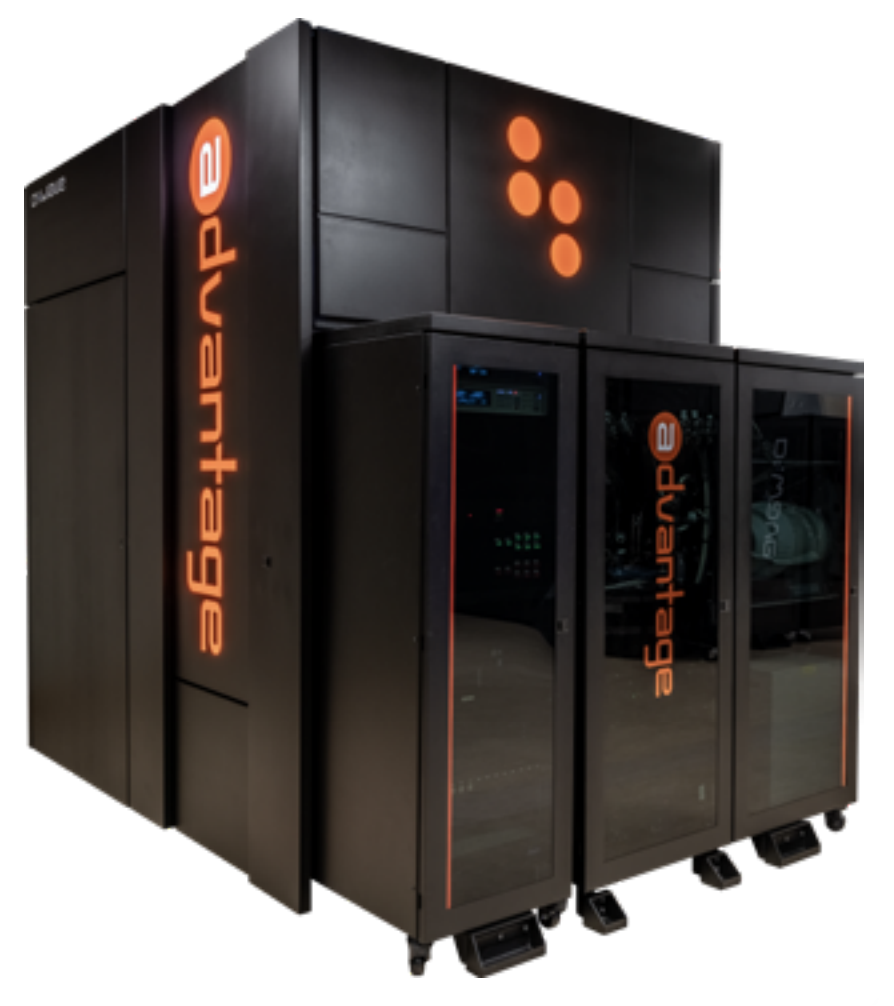
\includegraphics[scale=0.2]{Advantage.png}
			\end{minipage}
		\end{center}
		
	\end{frame}